\documentclass[a4paper,
fontsize=11pt,
%headings=small,
oneside,
numbers=noperiodatend,
parskip=half-,
bibliography=totoc,
final
]{scrartcl}

\usepackage{synttree}
\usepackage{graphicx}
\setkeys{Gin}{width=.6\textwidth} %default pics size

\graphicspath{{./plots/}}
\usepackage[ngerman]{babel}
%\usepackage{amsmath}
\usepackage[utf8x]{inputenc}
\usepackage [hyphens]{url}
\usepackage{booktabs} 
\usepackage[left=2.4cm,right=2.4cm,top=2.3cm,bottom=2cm,includeheadfoot]{geometry}
\usepackage{eurosym}
\usepackage{multirow}
\usepackage[ngerman]{varioref}
\setcapindent{1em}
\renewcommand{\labelitemi}{--}
\usepackage{paralist}
\usepackage{pdfpages}
\usepackage{lscape}
\usepackage{float}
\usepackage{acronym}
\usepackage{eurosym}
\usepackage[babel]{csquotes}
\usepackage{longtable,lscape}
\usepackage{mathpazo}
\usepackage[flushmargin,ragged]{footmisc} % left align footnote

\urlstyle{same}  % don't use monospace font for urls

\usepackage[fleqn]{amsmath}

%adjust fontsize for part

\usepackage{sectsty}
\partfont{\large}

%Das BibTeX-Zeichen mit \BibTeX setzen:
\def\symbol#1{\char #1\relax}
\def\bsl{{\tt\symbol{'134}}}
\def\BibTeX{{\rm B\kern-.05em{\sc i\kern-.025em b}\kern-.08em
    T\kern-.1667em\lower.7ex\hbox{E}\kern-.125emX}}

\usepackage{fancyhdr}
\fancyhf{}
\pagestyle{fancyplain}
\fancyhead[R]{\thepage}

%meta
%meta

\fancyhead[L]{H. Stadler, K. Schuldt \\ %author
LIBREAS. Library Ideas, 25 (2014). % journal, issue, volume.
\href{http://nbn-resolving.de/urn:nbn:de:kobv:11-100219329
}{urn:nbn:de:kobv:11-100219329}} % urn
\fancyhead[R]{\thepage} %page number
\fancyfoot[L] {\textit{Creative Commons BY 3.0}} %licence
\fancyfoot[R] {\textit{ISSN: 1860-7950}}

\title{\LARGE{Spurensuche: Bibliothekarinnen, Berufsgeschichte, Sprache in Nachrufen. Ein Dialog}} %title %title
\author{Heike Stadler \& Karsten Schuldt} %author

\usepackage[colorlinks, linkcolor=black,citecolor=black, urlcolor=blue,
breaklinks= true]{hyperref}

\date{}
\begin{document}

\maketitle
\thispagestyle{fancyplain} 

%abstracts

%body
\textbf{Heike Stadler (HS):} Der Grund, warum dieser Text jetzt
entsteht, ist eigentlich trivial. Im Frühjahr 2012, als ich von Potsdam
nach Berlin gezogen bin, führten mich Recherchen zu der Straße in der
ich wohne, zu der gußeisernen Tafel in der Rungestraße 25/27. Auf dieser
Tafel steht, dass in diesem Haus die Wirkungsstätte der ersten
Bibliothekarin in Deutschland, Bona Peiser, war. Ich wohnte also in
jener~ Straße, in der sich die erste Öffentliche Lesehalle Berlins
befand. Das fand ich als Bibliothekarin natürlich interessant. Der Name
Bona Peiser war mir bis dato nicht präsent. Na ja, jedenfalls habe ich
angefangen zu recherchieren. Im Rahmen meiner Recherchen erfuhr ich,
dass Frauke Mahrt-Thomsen ein Buch zu Bona Peiser verfassen wird.

Als das Buch erschien (Mahrt-Thomsen 2013), habe ich mich gefragt, warum
es jetzt im Untertitel heisst \enquote{Die erste deutsche
Bibliothekarin} und nicht, wie auf der Gedenktafel \enquote{die erste
Bibliothekarin Deutschlands}. Ist es wichtig? Ist es unwichtig, ob
jemand die erste deutsche Bibliothekarin oder die erste Bibliothekarin
in Deutschland war? Insbesondere wenn wir uns mit der Geschichte des
Bibliotheksberufes auseinandersetzen? Was sagst du dazu?

\textbf{Karsten Schuldt (KS):} Sprache ist immer wichtig. Sprache
konstituiert Wirklichkeit. Es lässt sich bei dieser Änderung tatsächlich
viel vermuten. War Bona Peiser keine Deutsche? War sie -- immerhin lebte
sie Anfang des 20. Jahrhunderts in Deutschland, in dem der
Antisemitismus virulent war -- Jüdin und deshalb von weiteren Teilen
nicht als Deutsche akzeptiert? Gab es vorher schon Deutsche, die
Bibliothekarinnen waren, in den Kolonien, im Ausland?

\textbf{HS}: Darauf kann ich jetzt erstmal nicht antworten. Wenn wir uns
mit der Geschichte des Bibliothekswesens befassen, will ich aber schon
wissen, wer sie genau war. War sie nun Volksbibliothekarin in Berlin,
wie sie Thomas Adametz (1987) bezeichnet hat? Ist sie Bibliothekarin in
Deutschland (Mahrt-Thomsen 1995)? Ist sie deutsche Bibliothekarin oder
ist sie Bibliothekarin in Deutschland? Ist sie Volksbibliothekarin oder
Bibliothekarin? Ist das ein wichtiger Unterschied oder nicht? Das zeigt
ja auch, auf wie wenig genaues wir im Bibliothekswesen uns bislang
geeinigt haben. Ich finde, im Sinne der Berufsgeschichte sollten wir da
schon etwas präziser sein.

\textbf{KS:} Man kann da einiges vermuten. Adametz hat seinen Text in
der DDR geschrieben, in einer Zeit, in der man von zwei deutschen
Staaten ausging. Mahrt-Thomsen schrieb nach der Wende. Genaueres muss
man in den Texten schauen.

Aber insgesamt wissen wir doch an sich wenig über die Geschichte des
Bibliotheksberufes. Wird darüber überhaupt diskutiert? In meiner
Ausbildung kam das, soweit ich mich erinnere, gar nicht vor. Nur als
Vergleich: In den Gender Studies, die ich gleichzeitig studierte, haben
wir viel über die Geschichte der Frauenbewegungen gehört, erste Welle,
zweite Welle, proletarische versus bürgerliche Frauenbewegung, in
unterschiedlichen Ländern und so weiter. Aber in der
Bibliothekswissenschaft, da waren die Bibliotheken einfach nur da.

\textbf{HS:} Um sich mit seinem Beruf gegebenenfalls identifizieren zu
können, sollte man sich in der Ausbildung schon mit der Geschichte
dieses Berufes auseinandersetzen. Vielleicht müssen wir da auch erstmal
einen Punkt machen und es müssen andere definieren, was sie ist:
Bibliothekarin? Volksbibliothekarin?

Was ich mich parallel frage: Hat jemand in anderen grossen deutschen
Städten -- Hamburg, Köln, München, Leipzig, Frankfurt/Main und so weiter
-- recherchiert, ob es da früher Bibliothekarinnen gab? Um sagen zu
können, dass Peiser die erste Bibliothekarin in Deutschland war, muss
man doch auch über die anderen Städte etwas recherchieren. Ich habe
weiter recherchiert zu Nachrufen von anderen Bibliothekarinnen. Bei
diesen bin ich auf keine andere Person gestossen, die das widerlegen
könnte, was aber nicht heisst, dass das damit bewiesen ist.

\textbf{KS:} Wie viel Nachrufe hast du denn überhaupt gefunden? Als ich
für den Call for Paper für die Frauen-Ausgabe recherchiert habe, ist mir
schon aufgefallen, dass es einen Haufen von Texten gibt, die sich mit
dem Thema befassen, bis hin zu empirischen und soziologischen Studien,
die aber nicht mehr referenziert werden. Das ist doch schon erstaunlich.

\begin{figure}[htbp]
\centering
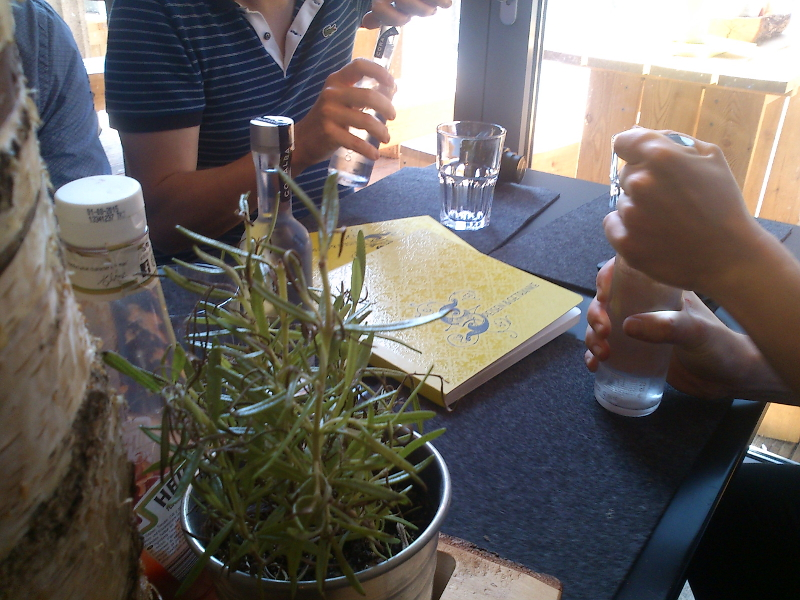
\includegraphics{editorialbild.jpg}
\caption{Redaktionsorte VI (Berlin-Mitte, Juli 2014)}
\end{figure}

\textbf{HS:} Nachrufe aus der Zeit, in der Bona Peiser gelebt hat, habe
ich nicht gefunden. Ich bin eher auf Nachrufe von Bibliothekarinnen
gestossen, die in den 1960ern und 70ern in den Fachzeitschriften
abgedruckt wurden. Nachrufe von Männern gab es wohl immer, die habe ich
beständig gefunden. Aber für Frauen habe ich die erst in den 1960er und
70ern gefunden.

\textbf{KS:} Das ist interessant, das geht doch einher mit der
feministischen Geschichtsschreibung, die sich auch in den 1960er und
1970er Jahren verstärkt für die Biographien einzelner Frauen
interessierte und versucht hat, diese Biographien von Männern gegenüber
zu stellen. Ich kann mir da gut eine Verbindung vorstellen, auch wenn
man heute im Bibliothekswesen nicht gerne über Politik und Gesellschaft
reden will. Hast du denn bei den Biographien Unterschiede festgestellt?

\textbf{HS:} Zumindest bei den Biographien, die in der ehemaligen DDR in
der Fachliteratur publiziert worden sind, wird mehr das Wirken im Rahmen
der beruflichen Tätigkeiten der Bibliothekarinnen für die Nachwelt
festgehalten, während ich den Eindruck habe, dass in den anderen
Biographien eher blumiger über die Bibliothekarinnen gesprochen wird.
Ich will nicht sagen, dass in Westdeutschland nicht über die Tätigkeiten
geschrieben wurde, aber es ist eine ganz andere Sprache. Lass mich ein
paar Beispiele geben.

Aus dem Nachruf für Lieselotte Stöhr (1976, DDR).

\begin{quote}
\enquote{Mit großem Engagement und Können setzte sie sich {[}\ldots{}{]}
für die Entwicklung eines sozialistischen Bibliothekswesens ein, dessen
Profil insbesondere in der Hauptstadt der DDR, Berlin, von ihr mit
geprägt wurde.} (Anonym 1976, S. 623)
\end{quote}

\begin{quote}
\enquote{Aus der fachlichen Arbeit erhielt sie Impulse für ihr
gesellschaftliches Wirken -- zum Beispiel als langjähriges Mitglieder
der Parteileitung unserer Bibliothek -- und aus der gesellschaftlichen
Tätigkeit erwuchsen der Fachreferentin für Gesellschaftswissenschaften
neue Ideen zum Nutzen der Leser.} (Anonym 1976, S. 623)
\end{quote}

\begin{quote}
\enquote{Für eine Bibliotheksöffentlichkeit im besten Sinne des Wortes
zu wirken, dafür scheute sie keine Mühe, keinen persönlichen Einsatz.}
(Anonym 1976, S. 623)
\end{quote}

Oder aus dem Nachruf für Ilse Korn (DDR, 1976).

\begin{quote}
\enquote{Ilse Korn war Bibliothekarin mit voller Hingabe an ihre
Erziehungs- und Bildungsaufgabe, sie übersah aber auch nicht die
organisatorischen Erfordernisse dieses Berufs.} (Müller-Muck 1976, S.
472)
\end{quote}

\begin{quote}
\enquote{Ilse Korn hatte mit Genehmigung der sowjetischen
Militäradminstration (SMA) und gefördert von Genossin Galina
Snimtschikowa den Entwurf eines Büchereigesetzes für das damalige
Sachsen erarbeitet, das u.a. die Grundlagen schaffen sollte, um in jeder
Ortschaft entsprechend der Einwohnerzahl eine Bibliothekseinrichtung zu
schaffen. Es ist verständlich und berechtigt, daß Ilse Korn auf diesen
Gesetzentwurf besonders stolz war.} (Müller-Muck 1976, S. 472)
\end{quote}

Und aus den Erinnerungen an Lotte Bergtel (DDR, 1966).

\begin{quote}
\enquote{Lotte Bergtel war eine leidenschaftliche Bibliothekarin. Sie
wußte von der großen Wirkung, die die Literatur bei der Entwicklung
allseitig gebildeter, sozialistisch denkender und handelnder Menschen
hat.} (Anonym 1966, S. 139)
\end{quote}

\begin{quote}
\enquote{Lotte Bergtel hat sich bei der Entwicklung unseres
Bibliothekswesens große Verdienste erworben. Sie zu ehren, ihr zu
gedenken, ist für uns alle eine natürliche Pflicht.} (Anonym 1966, S.
139)
\end{quote}

\begin{quote}
\enquote{Als Referentin im Berlin Magistrat war sie massgeblich am
Wiederaufbau des Berliner Volksbüchereiwesens beteiligt, leitete sie
Arbeitskreise mit dem Ziel nazistische Literatur zu entfernen,
humanistische Werke richtig und klar einzuschätzen und sinnvoll
einzusetzen. Ihre Hauptsorge aber galt der Ausbildung neuer,
fortschrittlicher Nachwuchskräfte, die bewußt als antifaschistische
Bibliothekare im Kampf um ein kommendes sozialistisches Deutschland ihre
politische Verantwortung erkannten und nie wieder zulassen würden, daß
die progressiven Werke der deutschen und Weltliteratur auf
Scheiterhaufen brennen und aus den Regalen der Bibliotheken entfernt
würden.} (Woita 1966, S. 141)
\end{quote}

Das sind alles große Sätze und ich habe den Eindruck, dass man die kaum~
im bibliothekswissenschaftlichen Kontext einordnen kann. War das Wirken
dieser Frauen so gross oder wurden sie durch den Nachruf -- insbesondere
im Rückblick, jetzt, 50 Jahre später, wo ich diese Sätze lese -- dazu
gemacht?

\textbf{KS:} Mir scheint das auch eine ganz schöne heftige DDR-Sprache
zu sein und es ist schwierig, da das Politische und die Realität
voneinander zu trennen. Wie sah es denn mit den Nachrufen im Westen aus?
Waren die auch so politisiert?

\textbf{HS:} Ja, stopp. Nur als Frage: Wie viele Biographien von Frauen
im Bibliothekswesen kennst du denn? Wir leben doch im Bibliothekswesen
oft nur im Jetzt.

\textbf{KS:} Wenige. Und die wenigen Nachrufe, die ich kenne, sind
eigentlich immer Männer, wie zum Beispiel letztens in der BuB
(11-12/2013), \enquote{Bedeutende Bibliothekare}. In einem
\enquote{Frauenberuf}. Das ist doch erstaunlich.

\textbf{HS:} Es ist schwer ein direktes Pendant für diese Sprache zu
finden. Aber dennoch ein paar Beispiele. Aus dem Nachruf für Anne
Walther von Walter Kolbe (BRD, 1974):

\begin{quote}
\enquote{Ihr berufliches Leben verkörperte wie das vieler
Bibliothekarinnen der Ersten Generation ein Stück Bibliotheksgeschichte.
Auch sie musste sich als ‚Tochter aus gutem Hause` ihren Beruf schwer
erkämpfen und hatte mit den damals üblichen Schwierigkeiten zu rechnen.}
(Kolbe 1974, S. 360)
\end{quote}

\begin{quote}
\enquote{Aus nächster Nähe erlebte sie den fachlichen
\enquote{Richtungsstreit} jener Jahre. Schwerlich können wir uns heute
noch das leidenschaftliche Engagement dieser Bibliothekare vorstellen
mit dem sie nach neuen Lösungen suchten und bibliothekstechnische
Verbesserungen erfanden. Von diesen Zeiten unter einem nüchternen und
liberalen Chef dessen Fähigkeiten zum Organisieren ihrer eigenen
speziellen Begabung entsprach berichtete Anna Walther immer mit
Begeisterung.} (Kolbe 1974, S. 360)
\end{quote}

\begin{quote}
\enquote{Jeder, der sie kannte, wird mit Respekt und Dankbarkeit an
diese herbe und dennoch gütige Kollegin denken.} (Kolbe 1974, S. 361)
\end{quote}

Was sagt uns das über Anne Walther? Wir wissen weder, welche Position
sie im \enquote{Richtungsstreit} einnahm, noch ob ihr Beruf auch
Berufung war.

\textbf{KS:} Also verschwinden im Osten wie auch im Westen die Frauen im
Bibliothekswesen hinter Plattitüden, nur hinter unterschiedlichen.

\textbf{HS:} Ich gebe dir mal noch zwei andere Beispiele, zum Vergleich.

Zum Beispiel im Nachruf für Martha Böhmer geht Rudolf Joerden mehr auf
den Berufsstand ein, als auf die Person Böhmer selber. (BRD, 1973) Und
es wird auch nicht klar, warum er überhaupt einen Nachruf für sie
schreibt.

\begin{quote}
\enquote{Marthe Böhmer war alles andere als ein theoretischer Mensch.
Von ihr wurden weder Aufsätze noch Rezensionen veröffentlicht, um so
seltsamer, als sie durch Jahrzehnte ausführliche Erinnerungsstützen
ihrer fleißigen Privatlektüre niederschrieb. Sie war -- als ob sie die
Verpflichtung ihres Vornamens einlösen wollte -- ein Mensch des
Zupackens, jederzeit diszipliniert, unsentimental und hilfsbereit
gegenüber jeder sich zeigenden Not, mit sicherem Gespür für das Mögliche
und Gemäße in das Leben anderer eingreifend, bei aller Höflichkeit
unbeeindruckt von irgendwelchen Würden ‚hochgestellter
Persönlichkeiten`, ohne jeden Hochmut, im Urteilen sicher und schnell,
in ihren Äußerungen unverblühmt und ohne Sinn für Diplomatie.} (Joerden
1973, S. 995)
\end{quote}

\textbf{KS:} Ja, das ist doch erstaunlich, oder? Sagt er überhaupt
irgendetwas Positives über sie oder sieht er sie als dankbares
Arbeitstier? Wenn das überhaupt etwas über die Zeit aussagt, scheint mir
vor allem, dass Frauen in Bibliotheken in den 1970ern geschätzt wurden,
wenn Sie viel arbeiteten und selber kaum ihre Meinung äusserten.
Zumindest, wenn man diesem Artikel folgt.

\textbf{HS:} Oder wenn man ihre Meinung kannte, schien es nicht wert,
sie festzuhalten.

\textbf{KS:} Aber nur als Nebenbemerkung: Rudolf Joerden war auch nicht
irgendjemand. Der hat im Nationalsozialismus zu völkischer
Bibliothekspolitik publiziert und dann offenbar einfach weiter
geschrieben. (Joerden 1939) Das scheint mir schon sehr zeittypisch zu
sein, dass er daseinfach tun konnte. Und Elisabeth Propach, von der du
auch einen Nachruf hast, hat auch 1939 eine Verwaltungslehre
veröffentlicht, dann 1950 wieder, ohne eine sichtbare Unterbrechung.
(Propach 1939, 1950) Das finde ich auch ganz schön erschreckend.

\textbf{HS:} Beim Nachruf für Elisabeth Propach ist ihr Wirken schon
beschrieben, aber es wird nicht deutlich, welche Bedeutung diese gehabt
haben könnte -- im Gegensatz zu den Beispielen aus der DDR. (BRD, 1985)

\begin{quote}
\enquote{Über einen Menschen etwas zu sagen, der sich stehts so
Zurücknahm, der immer bemüht war, zu versachlichen, ist schwer.} (Weimar
1985, S. 406)
\end{quote}

\begin{quote}
\enquote{Wir danken Elisabeth Propach, die ein Leben lang der Sache, der
bibliothekarischen Ausbildung diente, wir gedenken einer Lehrerin, die
auf das Menschliche zu hören verstand.} (Weimar 1985, S. 406)
\end{quote}

\textbf{KS:} Noch mehr Plattitüden.

\textbf{HS:} Welche Schlüsse soll man daraus ziehen? Wie soll man, wenn
man schon bei einem Buch zur ersten Bibliothekarin (Mahrt-Thomsen 2013)
so viele Fragen hat und dann noch solche Nachrufe findet, mit solchen
Plattitüden, bei denen wir die Richtigkeit nicht überprüfen können,
daraus etwas lernen? Wie soll man das Einordnen? Wie sollen wir da etwas
über unsere Berufsgeschichte sagen können?

\textbf{KS:} Sind wir also auf ein unerledigtes Problem gestossen, auf
eine Lücke? Konzentrieren wir uns im Bibliothekswesen immer wieder nur
auf die Bibliothek und Dinge, die zu lösen sind, aber stellen gar nicht
die Frage, wer die Bibliothek macht? Eigentlich wollten wir mit einer
Erkenntnis aus diesem Text herauskommen. Aber vielleicht ist diese Lücke
alles, was wir herausgefunden haben,~ dieses Fehlen der
Berufsgeschichte. Ich finde ja, dass es Parallelen zwischen politischer
Geschichte, zwischen der Geschichte der Frauenbewegungen und diesen
Texten aus der bibliothekarischen Fachpresse gibt; aber mir scheint, wir
wissen zu wenig, um das untersuchen zu können. Mich ärgert eher, was du
da gefunden hast.

\section*{Literatur}\label{literatur}

Adametz, Thomas / Bona Peiser -- Berlins erste Volksbibliothekarin. In:
Der Bibliothekar 41 (1987), S.111-113

Andrae, Friedrich / Ursula von Dietze zum Gedenken (1925-1979). In: Buch
und Bibliothek 31 (1979) 7/8, S. 686

Anonym / Lotte Bergtel -- Erinnerungen ihrer Freunde {[}Einleitung{]}.
In: Der Bibliothekar 20 (1966) 2, S. 139-140

Anonym / Zum Tode von Lieselotte Stöhr. In: Der Bibliothekar 30 (1976)
9, S. 623-624

Beyersdorff, Günter / Nachruf für Professor Ilse Reichel. In: Buch und
Bibliothekar 27 (1975), S. 614-616

Deicke, Hanna / Nachruf für Annedore Weitbrecht. In: Buch und Bibliothek
30 (1978) 4, S. 268

Endell, Frida / Therese Krimmer †. In: Bücherei und Bildung 19 (1967),
S. 183-184

Joerden, Rudolf / Die Freihand in der Großstadt, ihre Werbekraft und
Reichweite bei Erwachsenen. In: Die Bücherei 6 (1939) 7/8 , S. 411-423

Joerden, Rudolf / Abschied von Martha Böhmer. In: Buch und Bibliothek 25
(1973) 1, S. 995

Kolbe, Walter / Nachruf auf Anne Walther. In: Buch und Bibliothek 26
(1974) 3, S. 360-361

Kuckhoff, Greta / Begegnung mit Lotte Bergtel. In: Buch und Bibliothek
20 (1966) 2, S. 142-143

Mahrt-Thomsen, Frauke / Bona Peiser: Die erste deutsche Bibliothekarin.
Wegbereiterin der Bücher- und Lesehallen-Bewegung und der Frauenarbeit
in Bibliotheken, Berlin : BibSpider, 2013

Mahrt-Thomsen, Frauke / \enquote{Die öffentliche Bibliothek muss
jederzeit für jedermann unentgeltlich offenstehen.} Bona Peiser --
Deutschlands erste Bibliothekarin. In: BuB 47 (1995) 1, S. 56-60

Müller-Muck, Helmut: Dem Gedenken Ilse Korns. In: Der Bibliothekar 30
(1976) 7, S471-472.

Peter, Heinz / Lotte Bergtel und die Berliner Büchereischule. In: Der
Bibliothekar 20 (1966) 2, S. 143-147

Propach, Elisabeth / Kurze Verwaltungslehre für die Städtische
Volksbücherei. Leipzig : Einkaufshaus für Büchereien, 1939

Propach, Elisabeth / Kurze Verwaltungslehre für die Städtische
Volksbücherei. Hamburg : Verlag Eberhard Stichnote, 1950

Scherf, Walter / Zum Tode Jella Lepmans. In: Bücherei und Bildung 22
(1970), S. 469-470

Siering, Elfriede / Gedenkfeier für Lotte Bergtel. In: Der Bibliothek 27
(1973) 9, S. 607-609

Steinhoff, Maria / Elisabeth Greulsberg 20.11.1901-20.11.1968. In:
Bücherei und Bildung 21 (1969), S. 72

Weimar, Volker / Nachruf für Elisabeth Propach. In: Buch und Bibliothek
27 (1985), S. 406-407

Woita Irene / Würdige Ehrung einer verdienstvollen Bibliothekarin. In:
Der Bibliothekar 20 (1966) 2, 140-142

%autor
\begin{center}\rule{3in}{0.4pt}\end{center}

\textbf{Heike Stadler} und \textbf{Karsten Schuldt} sind Mitglieder der
Redaktion der LIBREAS. Library Ideas.

\end{document}
